% Appendix: sparse wall-pressure sensing detail, v3 (Session 33 / D247).
% Rewritten on the v2.2 pooled artifacts (track_o1_recovery, track_t grid,
% envelope + family audit); the previous version carried v2.1 d=64 spatial
% numbers whose recovery ordering CONTRADICTED Section 4.3 (predictive most
% recoverable there; fukami most recoverable here) -- that split-brain is the
% audit finding this rewrite removes. Every number is a macros_v3 macro.

\rb{K}{APB-01}{States the sensing conventions and how the recovery estimator is selected. Needed before any recovery number can be read.}At deployment the vorticity field is not available; only the wall pressure is.
This appendix records the sensing conventions behind \S\ref{sec:res_wall} and
\S\ref{sec:res_tracking} and the placement-robustness checks that the main text
summarises. The input throughout is the span-averaged pressure on the $192$
surface taps; the recovery estimator is selected per family by encounter-grouped
cross-validation among a kernel-ridge regressor on the flattened window, a
multilayer perceptron, and a recurrent network over the window sequence, and the
recovered state is read by the same frozen probes as everywhere else.\re

\subsubsection*{Placement, and why it does not drive the ordering}
\rb{K}{APB-02}{Why the ordering is not an artefact of model-conditioned placement, with the target-blind rerun. Answers a real objection.}Two placements are used, deliberately. The filter and the recovery of
table~\ref{tab:recovery} sense at each family's own model-conditioned taps, the
greedy selection that best exposes that family's latent, because the estimator
comparison should give every family its best sensing. The delay-trade grid of
\S\ref{sec:res_delays} instead uses a single target-blind array, the QR-pivot
optimum of the wall-pressure modes \citep{manohar2018sensors}, nested so that
every tap count is a prefix of the next, because a sensor-budget claim must not
depend on a placement tuned to any model. The two meet where their sensing
coincides: the grid's eight-tap, thirty-frame cell rerun on the
model-conditioned taps closely reproduces the table's recovery
($\TbridgeState$). The energy-versus-information split of \S\ref{sec:res_wall}
is also placement-robust: under the shared target-blind array with the
kernel-ridge estimator alone, the reconstructive state remains the most
recoverable in variance ($\WqStateFukami$ against $\WqStateJepa$ for the
predictive and $\WqStatePod$ for the linear basis) and the predictive state
retains the most recoverable physics ($\WqObsJepa$ against $\WqObsFukami$ and
$\WqObsPod$), so neither ordering is an artefact of the model-conditioned
placement.\re

\subsubsection*{What the window recovers that the instant cannot}
\rb{T}{APB-03}{Restates the window-against-instant result already given in S4-20 and S4-21, with the same macros. The appendix adds only the enstrophy figure.}At a single frame the wall is blind to the wake-circulation direction of the
predictive state (\S\ref{sec:res_wall}); over the thirty-frame window the blind
coordinate becomes partially recoverable ($\ToneCircNegWThirty$ held-out, from
near zero at one frame), and the wake enstrophy read through the recovered state
reaches $\ToneEwWThirty$. The window, not the tap count, is what carries this:
the same quantities barely move as taps are added at a fixed single frame. This
is the delay-coordinate content of the sensing result, quantified in the grid of
\S\ref{sec:res_delays}; it is a statement about the static reconstruction, and
the filter inherits the sequential version of it through its assimilation
window rather than through any explicit delay embedding.\re

\subsubsection*{The recovered field}
\rb{K}{APB-04}{Reads the recovered-field panels and localises the loss to the wake structures. Connects the sensing result to physical space.}Decoding the pressure-recovered state through each family's diagnostic decoder
makes the recovery visible in physical space
(figure~\ref{fig:field_recovery}). The comparison within each row, recovered
field against that family's own decode ceiling, isolates the pressure step from
the decoder's reconstruction limit: the loss from ceiling to recovery is the
part attributable to the eight-tap window, and the panels show it concentrating
in the wake structures rather than in the near-body field, consistent with the
wall reading the force-carrying directions best (\S\ref{sec:res_wall}).\re

\begin{figure}
  \centering
  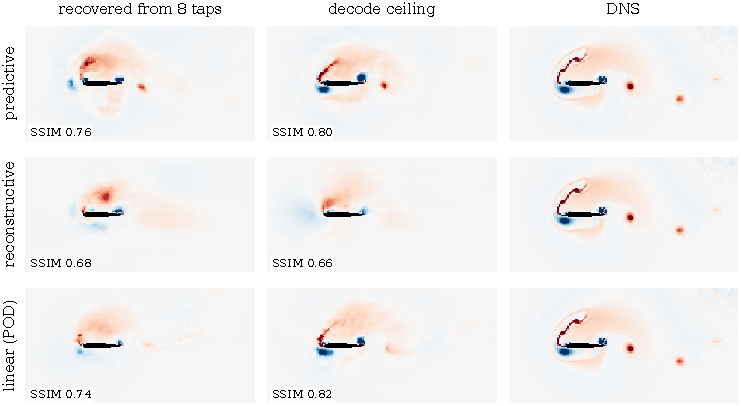
\includegraphics[width=\linewidth]{sections/figures/results/fig_field_recovery_v3.pdf}
  \caption{\rb{K}{APB-C1}{The recovered field against each family's own decode ceiling, which is the only fair comparison. The caption says so.}Flow recovered from eight wall-pressure taps on the representative
  held-out encounter of figure~\ref{fig:hero}, at the impact-side frame, one row
  per family. Columns: the field decoded from the pressure-recovered coefficient
  state, the decode ceiling (the same decoder applied to the encoded state, no
  pressure step), and the simulation; per-panel structural similarity annotated.
  The comparison is within each row, since the decoders' ceilings differ
  (\S\ref{sec:disc_decode}); the ceiling-to-recovered gap is the cost of the
  pressure step.\re}
  \label{fig:field_recovery}
\end{figure}

\subsubsection*{The out-of-distribution boundary from the sensing side}
\rb{T}{APB-05}{Restates the boundary failure of every static approach, already carried by S4-25 and table 12. The appendix repeats the numbers without adding evidence.}At the $|G| = 4$ boundary every static approach fails on the load, the
via-latent recovery at $\VrecCLGFour$ and the direct no-latent regression at
$\DirectCLKeightGFour$ from the same taps ($\DirectCLAllTapsGFour$ with the full
array), while the nonlinear filters still track it (table~\ref{tab:family_filter}). The
boundary is the same larger three-dimensional content the field carries there
(\S\ref{sec:flow_physics}): the mid-plane state captures less of the dynamics, so
a \StaticInv{} recovers little from a single instant, and only the accumulated
pressure history carries the load through.\re

\subsubsection*{Delay-coordinate knobs}
\rb{K}{APB-06}{Justifies the delay stride and window as convention rather than tuning, and declines the false-nearest-neighbours criterion honestly. Methodologically careful.}The window sweeps of \S\ref{sec:res_delays} keep the delay stride at the cache
cadence ($\Delta t = \DtTc\,c/u_\infty$), and this choice is a convention rather
than a tuning: the first minimum of the time-lagged mutual information of the
tap signals \citep{fraser1986} sits near $\TmiTau$ frames, about one shedding
period, so the thirty-frame window spans roughly one decorrelation time of the
wall pressure at the cadence used. The window length itself is selected by the
measured recovery trade rather than by a false-nearest-neighbours criterion
\citep{kennel1992}, which we regard as a cross-check and not a design input: the
delay-embedding guarantees are generic, wall pressure is a physical and
non-generic observable strongly coupled to the near-body vorticity, and the
operative evidence is the measured recovery, with the theorem as the organising
principle rather than a proof that a given tap count suffices.\re

\subsubsection*{Streaming deployment realism and the four-coefficient filter}

% Moved from Results (Session 39, D-B): the streaming realism and d=4 filter
% panels leave the main text with the estimator ladder.
\rb{K}{APB-07}{The streaming realism protocol and the four-coefficient filter, both demoted from \S4.6. Real results, correctly placed.}Under a deployment-realism protocol, streaming multi-encounter assimilation with
a pressure-only initialisation and no oracle anywhere, the filter on the
\PredState{} holds an impact-phase lift closure of \PoneStreamCleanZero{} on
clean taps and \PoneStreamCleanFive, \PoneStreamCleanTen{} and
\PoneStreamCleanTwenty{} at five, ten and twenty per cent tap noise (three
member-noise seeds each, figure~\ref{fig:deploy}). The four-dimensional
lift-critical state of \S\ref{sec:res_dimension} supports a filter of its
own at \PoneDFourFilterImpact{} impact median over five seeds, so a
four-coefficient state is estimable from the wall as well as forecastable.\re

\begin{figure}
  \centering
  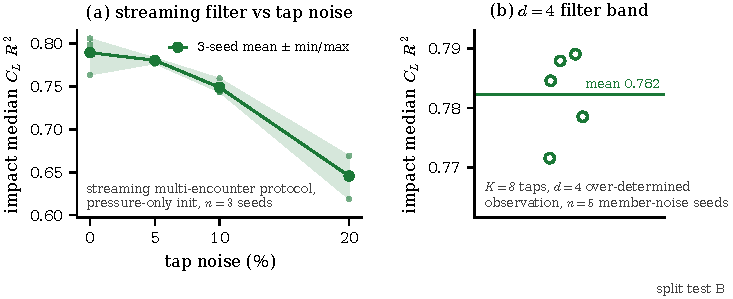
\includegraphics[width=0.9\linewidth]{sections/figures/results/fig_deployment_v4.pdf}
  \caption{\rb{K}{APB-C2}{The deployment-realism panels with the seed counts. Self-contained.}Deployment realism (\TestSplit{} set): (a)~streaming multi-encounter
  filter against tap noise, three member-noise seeds, validation-selected
  band (no test-set reference);
  (b)~the $d = 4$ filter band over five member-noise seeds.\re}
  \label{fig:deploy}
\end{figure}

% Moved from Results (Session 39, figure pass): the scale-invariance panel is an
% envelope diagnostic; the main-text sentence (\S\ref{sec:res_estimation}) points here.
\begin{figure}
  \centering
  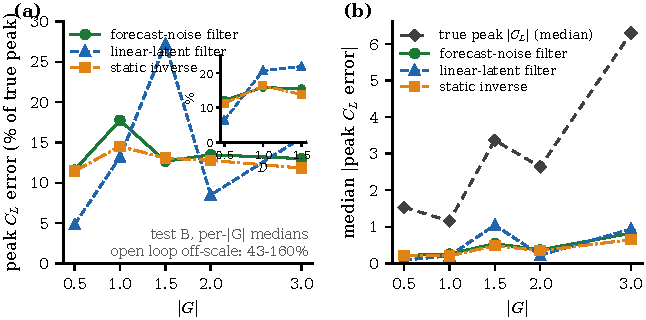
\includegraphics[width=0.9\linewidth]{sections/figures/results/fig_relative_errors_v4.pdf}
  \caption{\rb{K}{APB-C3}{Relative peak error across the envelope, the scale-invariance exhibit \S4.6.3 points at. Self-contained.}Relative peak error across the gust envelope (\TestSplit{} set,
  medians per $|G|$): the forecast-derived filter stays near
  $12$ to $14$ per cent at all but the $|G| = 1$ stratum while the linear
  filter is non-uniform; the
  absolute peak error (right) grows with the peak itself.\re}
  \label{fig:relerr}
\end{figure}

% Moved from Results (Session 39 figure pass): the per-family end-to-end sweeps.
\begin{figure}
  \centering
  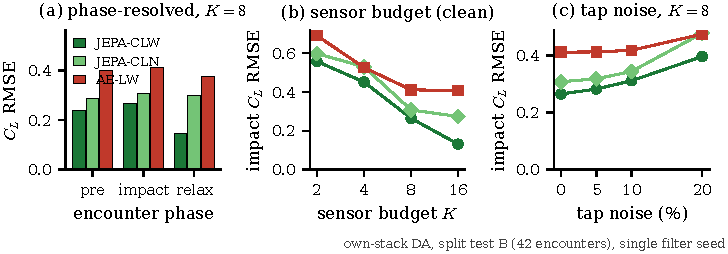
\includegraphics[width=\linewidth]{sections/figures/results/fig_ownstack_da_v4.pdf}
  \caption{\rb{K}{APB-C4}{The per-family end-to-end sweeps behind the own-stack claim. Single-seed provenance disclosed.}Per-family end-to-end comparison (\TestSplit{} set, $42$ encounters,
  single filter seed): (a)~phase-resolved lift error per family;
  (b)~sensor-budget sweep on each family's own nested placement;
  (c)~tap-noise sweep at $K = 8$.\re}
  \label{fig:ownstack}
\end{figure}

\subsubsection*{Choosing among the estimators}
\label{sec:disc_choosing}

% Moved from Discussion (Session 39, D-B): the estimator-selection guidance
% lives with the sensing appendix in the comparison-led revision.
\rb{K}{APB-08}{Explicit estimator-selection guidance in the Gupta idiom, ending in one sentence a practitioner can act on. The most useful paragraph in the appendices.}The ladder of \S\ref{sec:res_da} supports explicit selection guidance
\citep{gupta2026}. When only the in-distribution median matters and latency is
irrelevant, the \StaticInv{} is the strongest and simplest tool; the moment the
tails, the extrapolation boundary or continuous state tracking matter, the filters
take over, the \TwoStageKF{} online and the closed-form fixed-lag smoother on the
linear stack within a quarter-convective-time latency budget, while sparse or
intermittent pressure favours the linear filter with encoded observations (the
only member with zero consistency failures under subsampled updates). Across model
families the guidance is one sentence: anchored latent geometries, predictive or
linear, can be selected on dimension and budget alone, while unanchored
reconstructive geometries require a per-configuration estimatability check that
their probes do not predict.\re
